Here we include entity-relationship diagrams (ERDs) that focus on subsets of the database, to better explain the one-to-many and one-to-one connections between tables in the database. A table is indicated by a box (the name of the table is in the header), and connections between tables are indicated by dotted lines. A dotted line with a dot at either end indicates a \textbf{one-to-one} relationship, meaning that the rows in one table map perfectly onto the rows in the other table without overlap. A dotted line with a fork at one end indicates a \textbf{one-to-many} relationship, where the rows of the ``one'' table potentially map onto several rows of the ``many'' table.

\subsection*{Patent Attributes}

As seen below, each patent has a one-to-many relationship with its citations, classes, claims and application records. Citations (\verb`uspatentcitation`, \verb`foreigncitation`, \verb`usapplicationcitation` and \verb`otherreference`) are listed in the database in the same order they are listed in the patent file (as indicated by the \verb`sequence` column in those tables). This is also the case for claims in the \verb`claim` table. Patent classifications exist in the \verb`uspc` table, and are listed in order by the \verb`sequence` column, separated into main- and sub-classifications. Each patent also has an entry in the \verb`application` table, which contains metadata about the related application for the granted patent document, including filing date and application number. This application number can be used as a foreign key into the application database to obtain information for the inventors, claims, etc listed on the application document.

\begin{figure*}[!htbp]
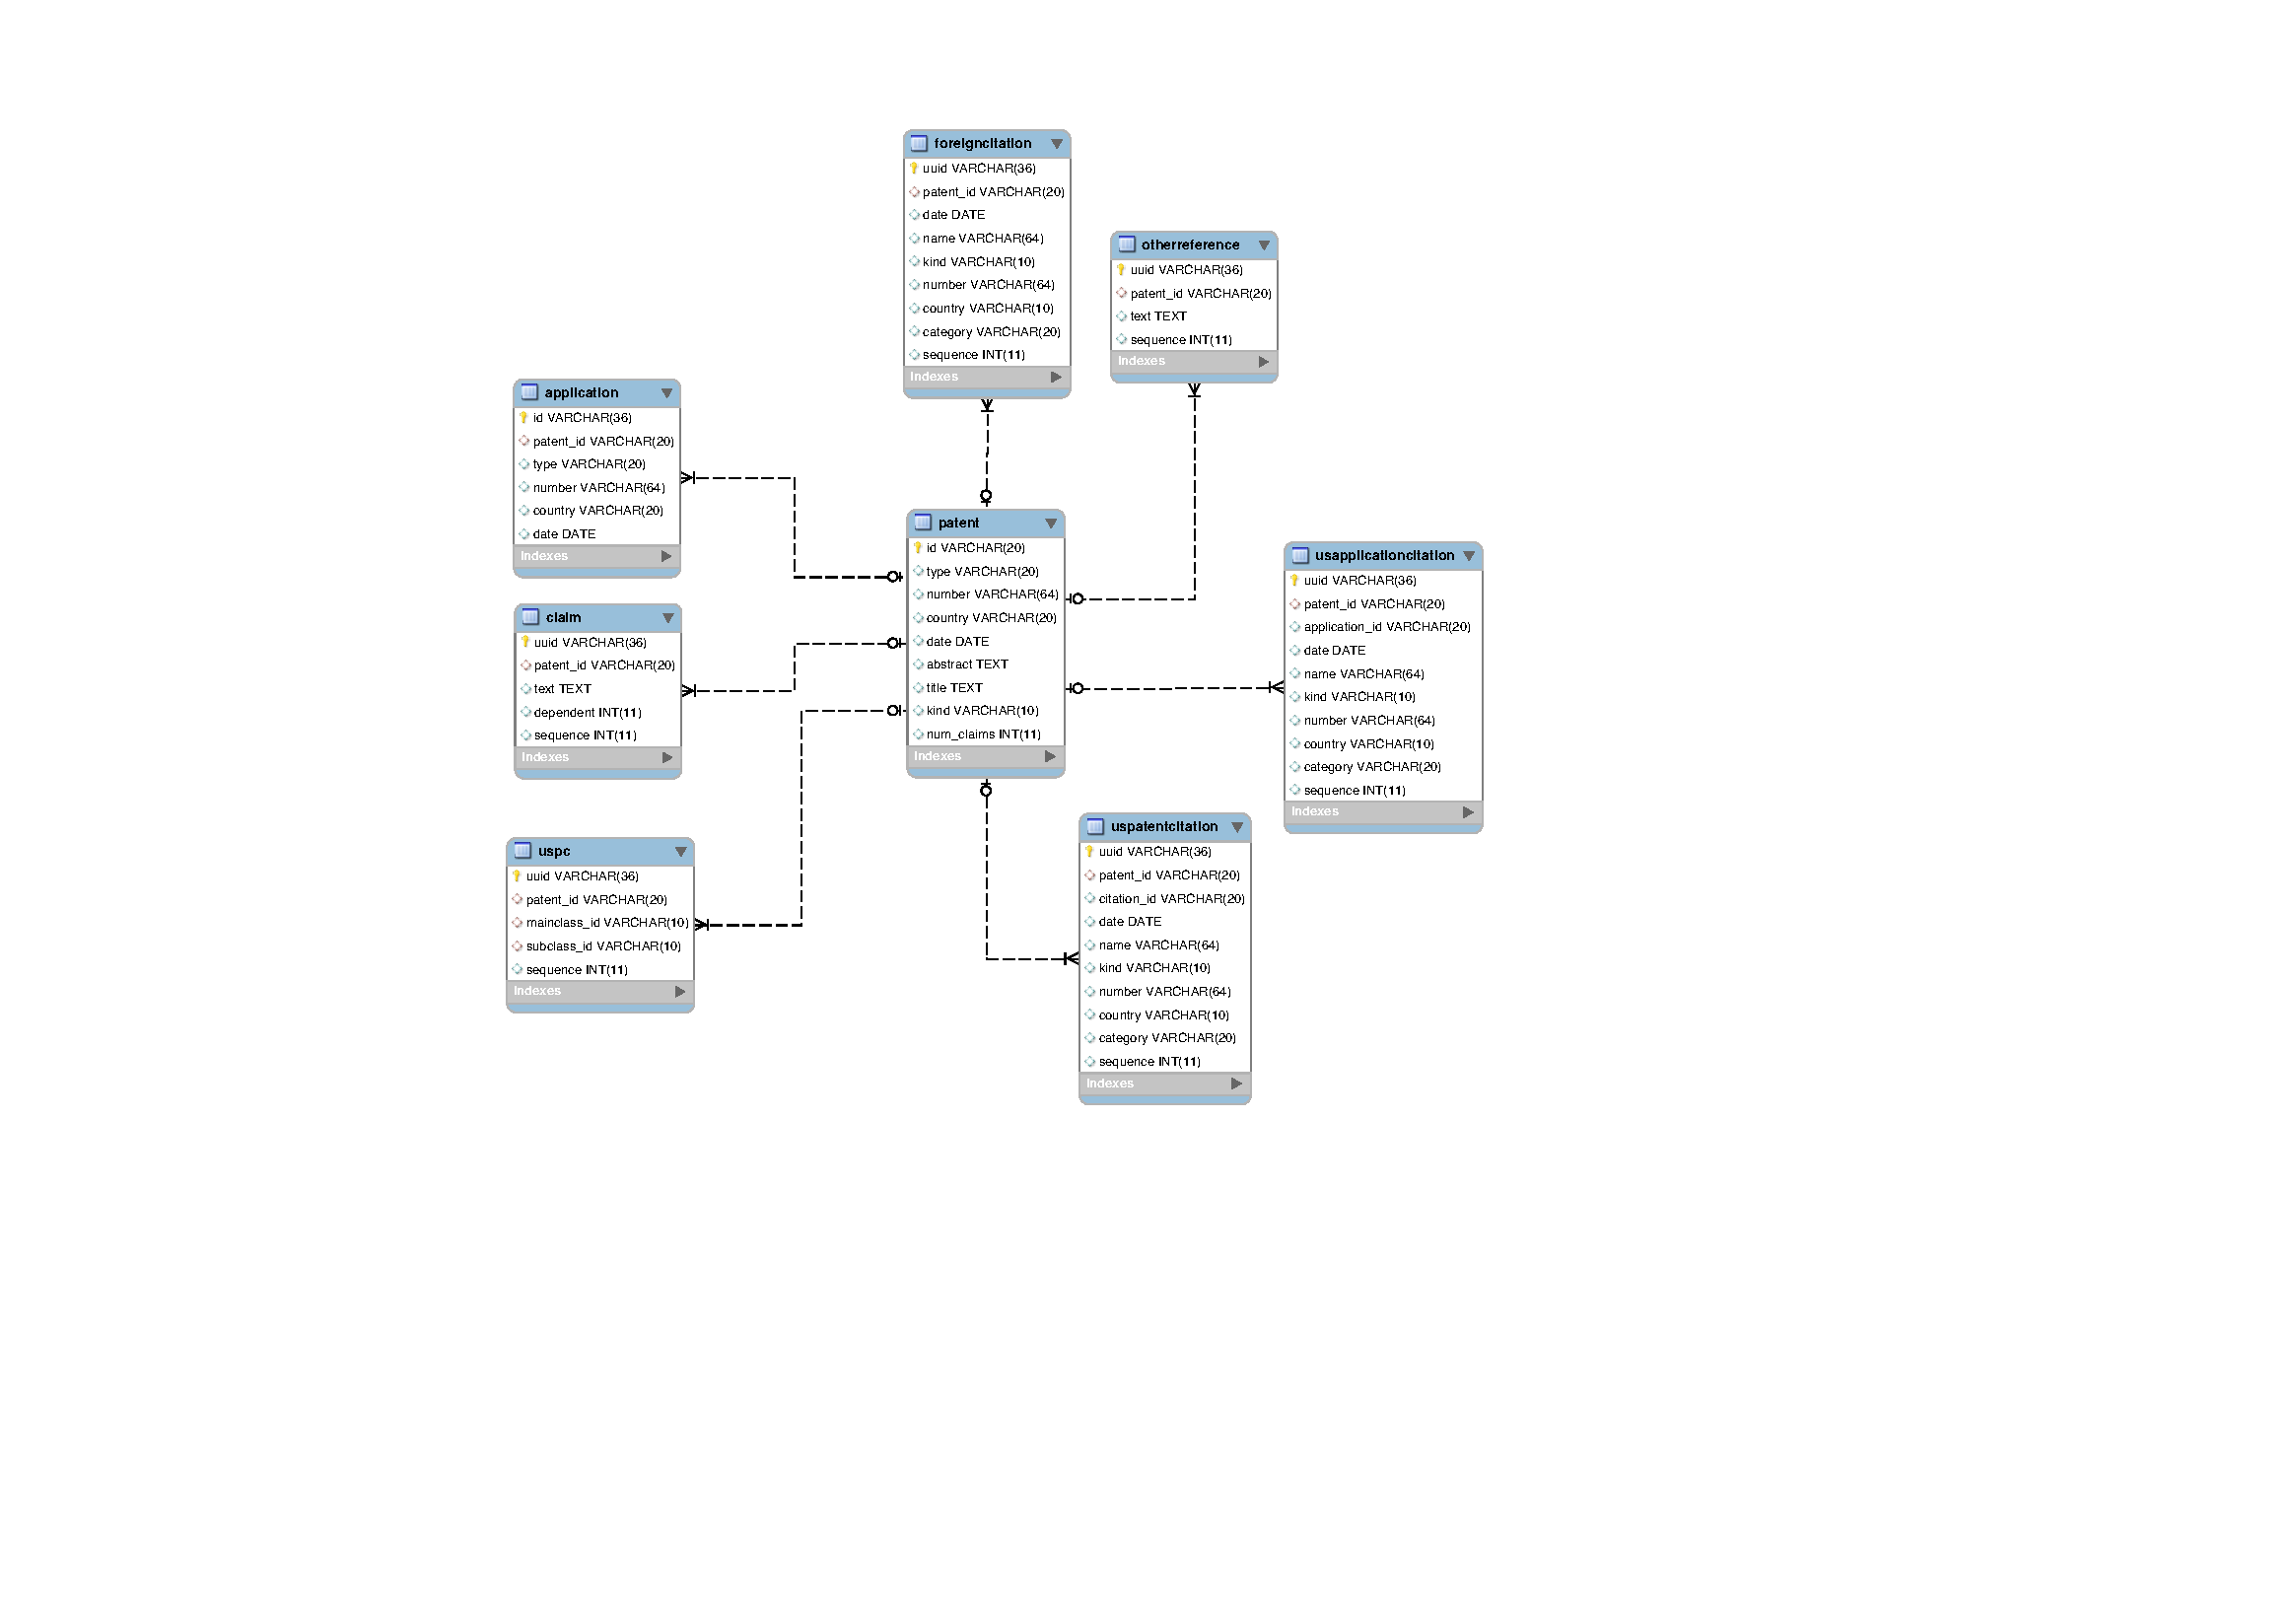
\includegraphics[width=\linewidth]{figs/Patentattributes}
\caption{Patents with citations, claims, applications and classes}
\end{figure*}

\subsection*{Patent Entities}

Here we explore the relationships between patents and inventors, lawyers and assignees.  Patents have \emph{many} \verb`rawlawyer`s, \verb`rawinventor`s and \verb`rawassignee`s. These relations are pulled directly from the USPTO XML files, that is, an instance of a \verb`rawinventor` belongs to a particular instance of a \verb`patent`, and no other records. As we will explore below, each of the \verb`rawlawyer`, \verb`rawinventor` and \verb`rawassignee` records is linked to a disambiguated record of the same type (\verb`rawassignee` to \verb`assignee`, for example).

\begin{figure*}[!htbp]
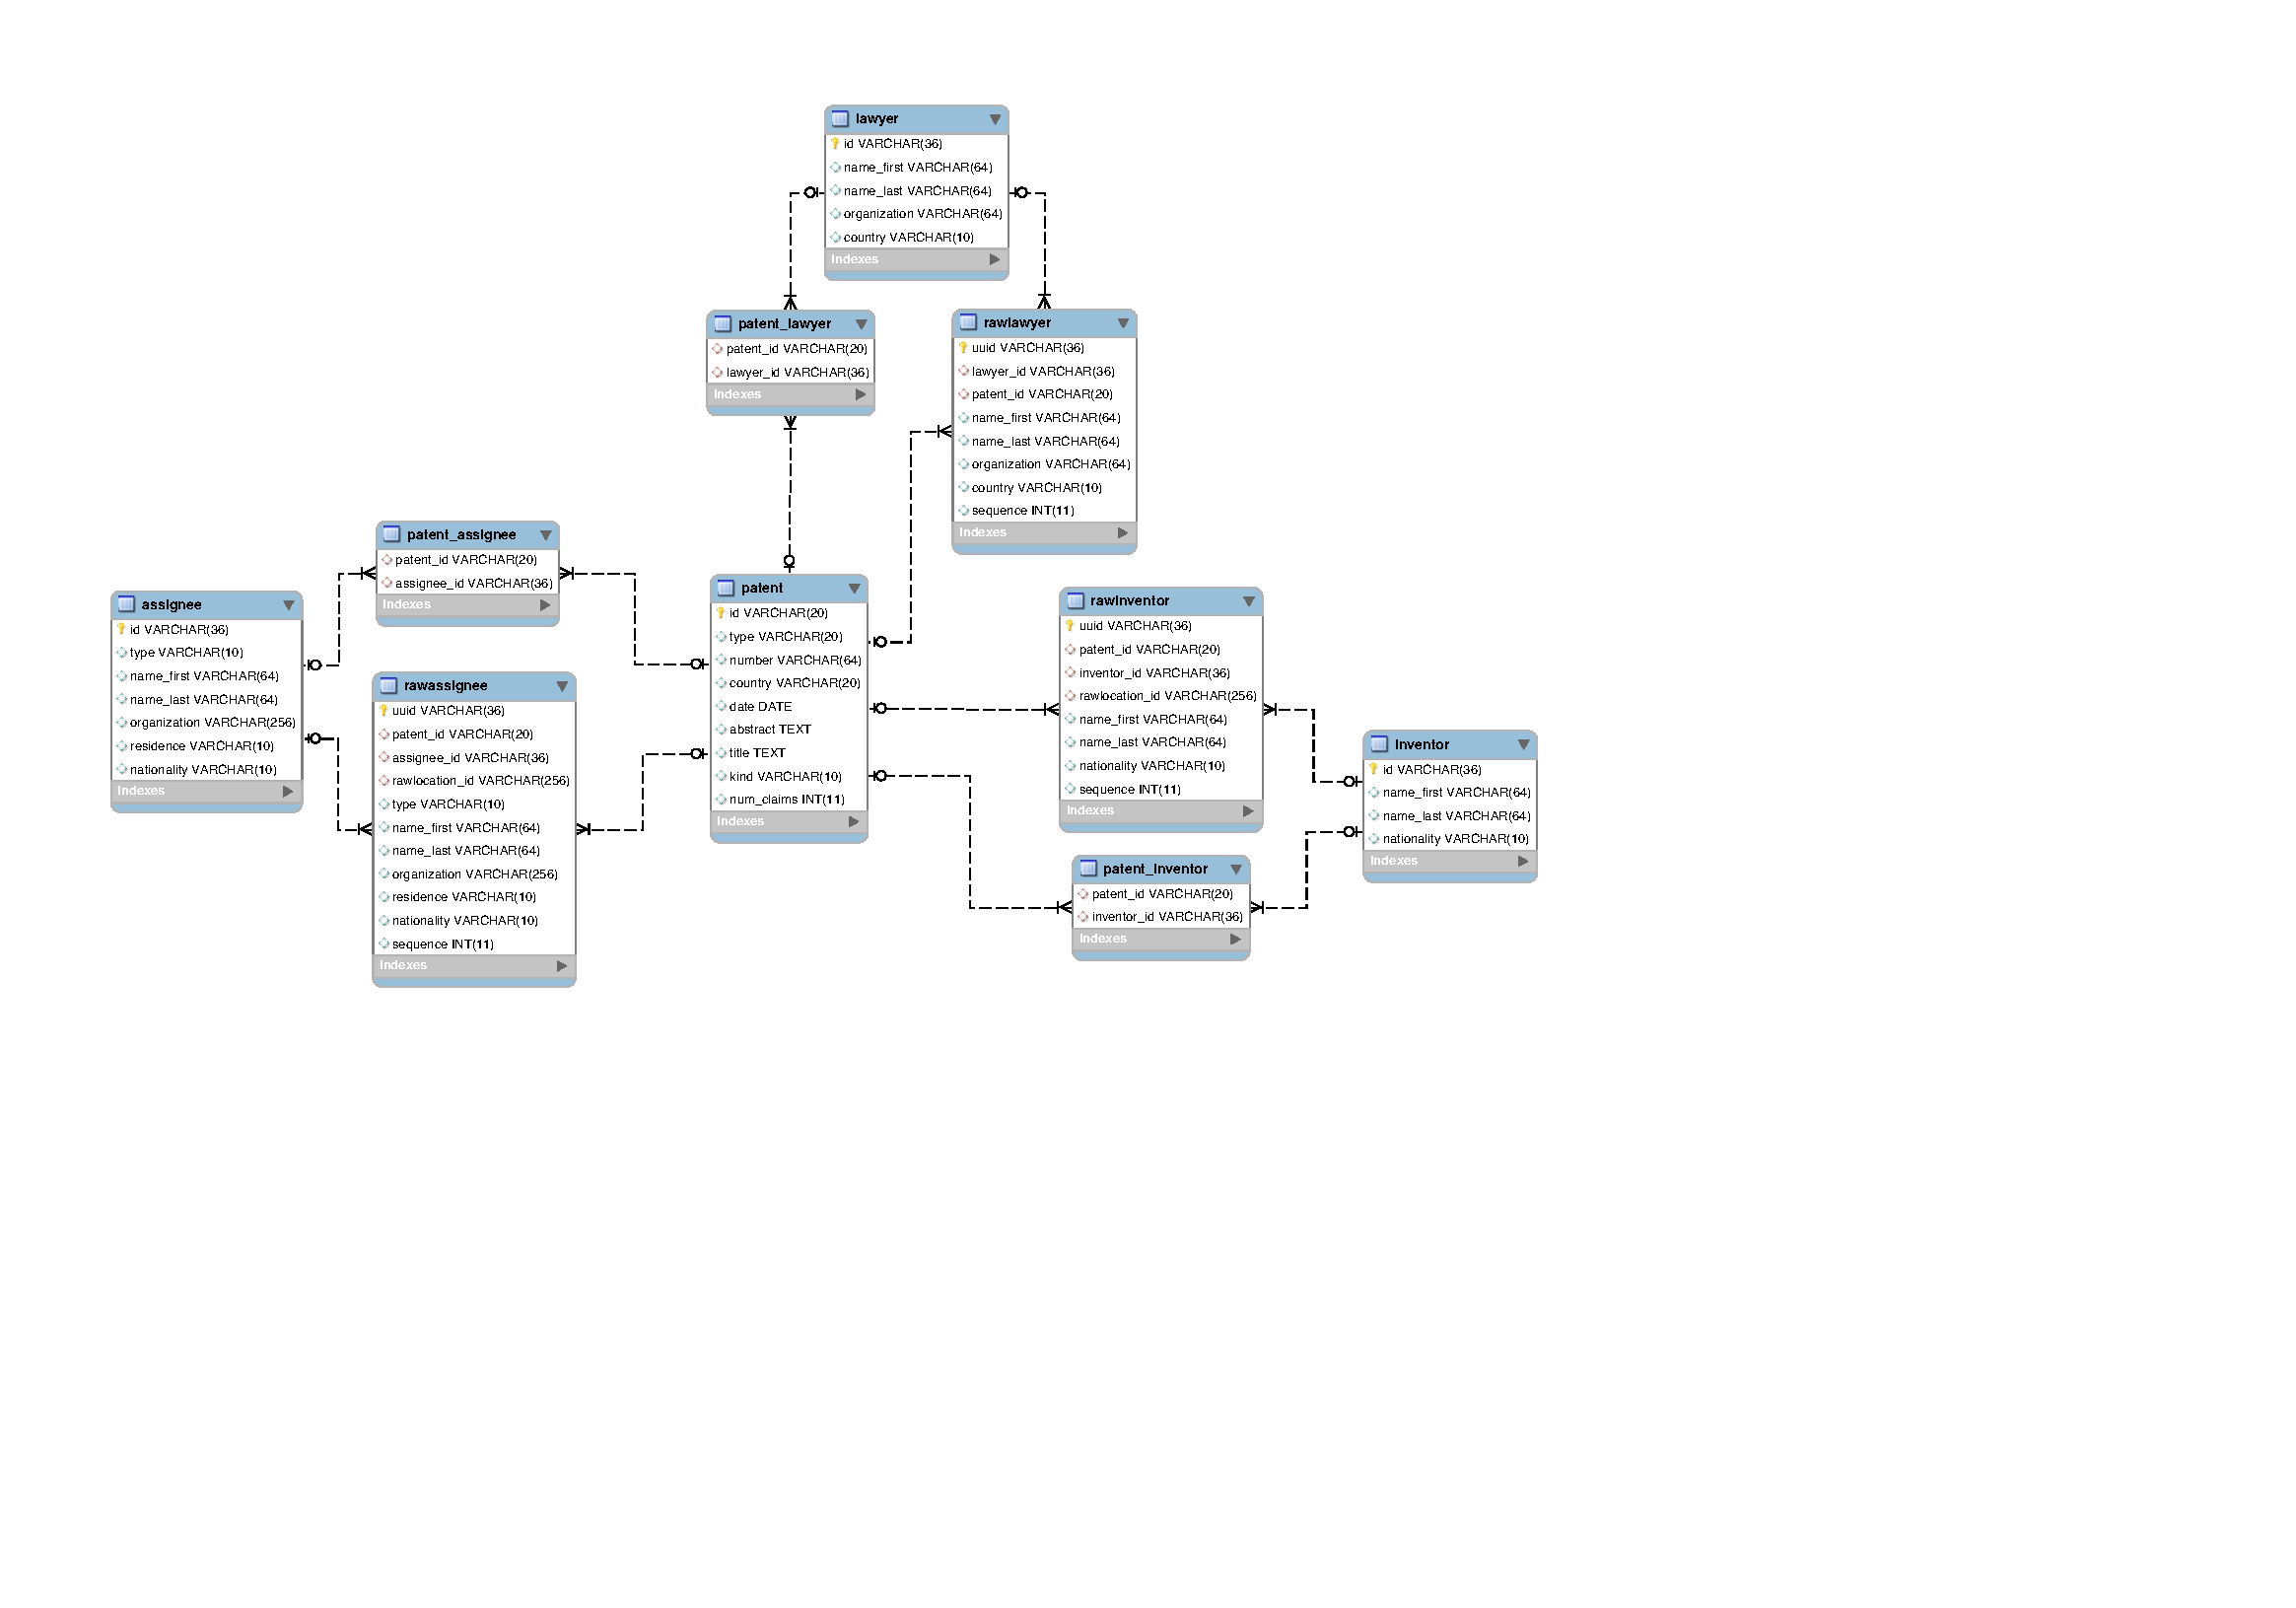
\includegraphics[width=\linewidth]{figs/Patententities}
\caption{Patents with Inventors, Assignees and Lawyers}
\end{figure*}

\subsection*{Inventors}

Expanding upon the patent-entity diagram above, we look at how inventor-related records are treated in the database. Patents have multiple inventors (order is, again, indicated by the \verb`sequence` column in the \verb`rawinventor` table) that are placed in the \verb`rawinventor` table. When the inventor disambiguation is run, each \verb`rawinventor` is linked with a disambiguated \verb`inventor` record in the \verb`inventor` table. As indicated in the ERD below, multiple \verb`rawinventor`s can be associated with a single \verb`inventor`. Each \verb`rawinventor` record also has a \verb`rawlocation` record, which is the location of that inventor as listed on the associated patent. Likewise, each \verb`rawlocation` is linked with a disambiguated \verb`location` record in the \verb`location` table after the geolocation disambiguation is performed. The linking table \verb`location_inventor` maintains the \verb`rawinventor-rawlocation` pairing, but uses the disambiguated records instead. Currently, the table contains all unique pairs of \verb`inventor` and \verb`location` as listed together on a patent document, in the order from oldest patent to newest patent. Keep in mind that because not all raw locations have disambiguated locations, not all inventors will have disambiguated locations.The \verb`patent_inventor` linking table mirrors the relationship of \verb`rawinventor` to \verb`patent`, but uses the disambiguated inventor record.

\begin{figure*}[!htbp]
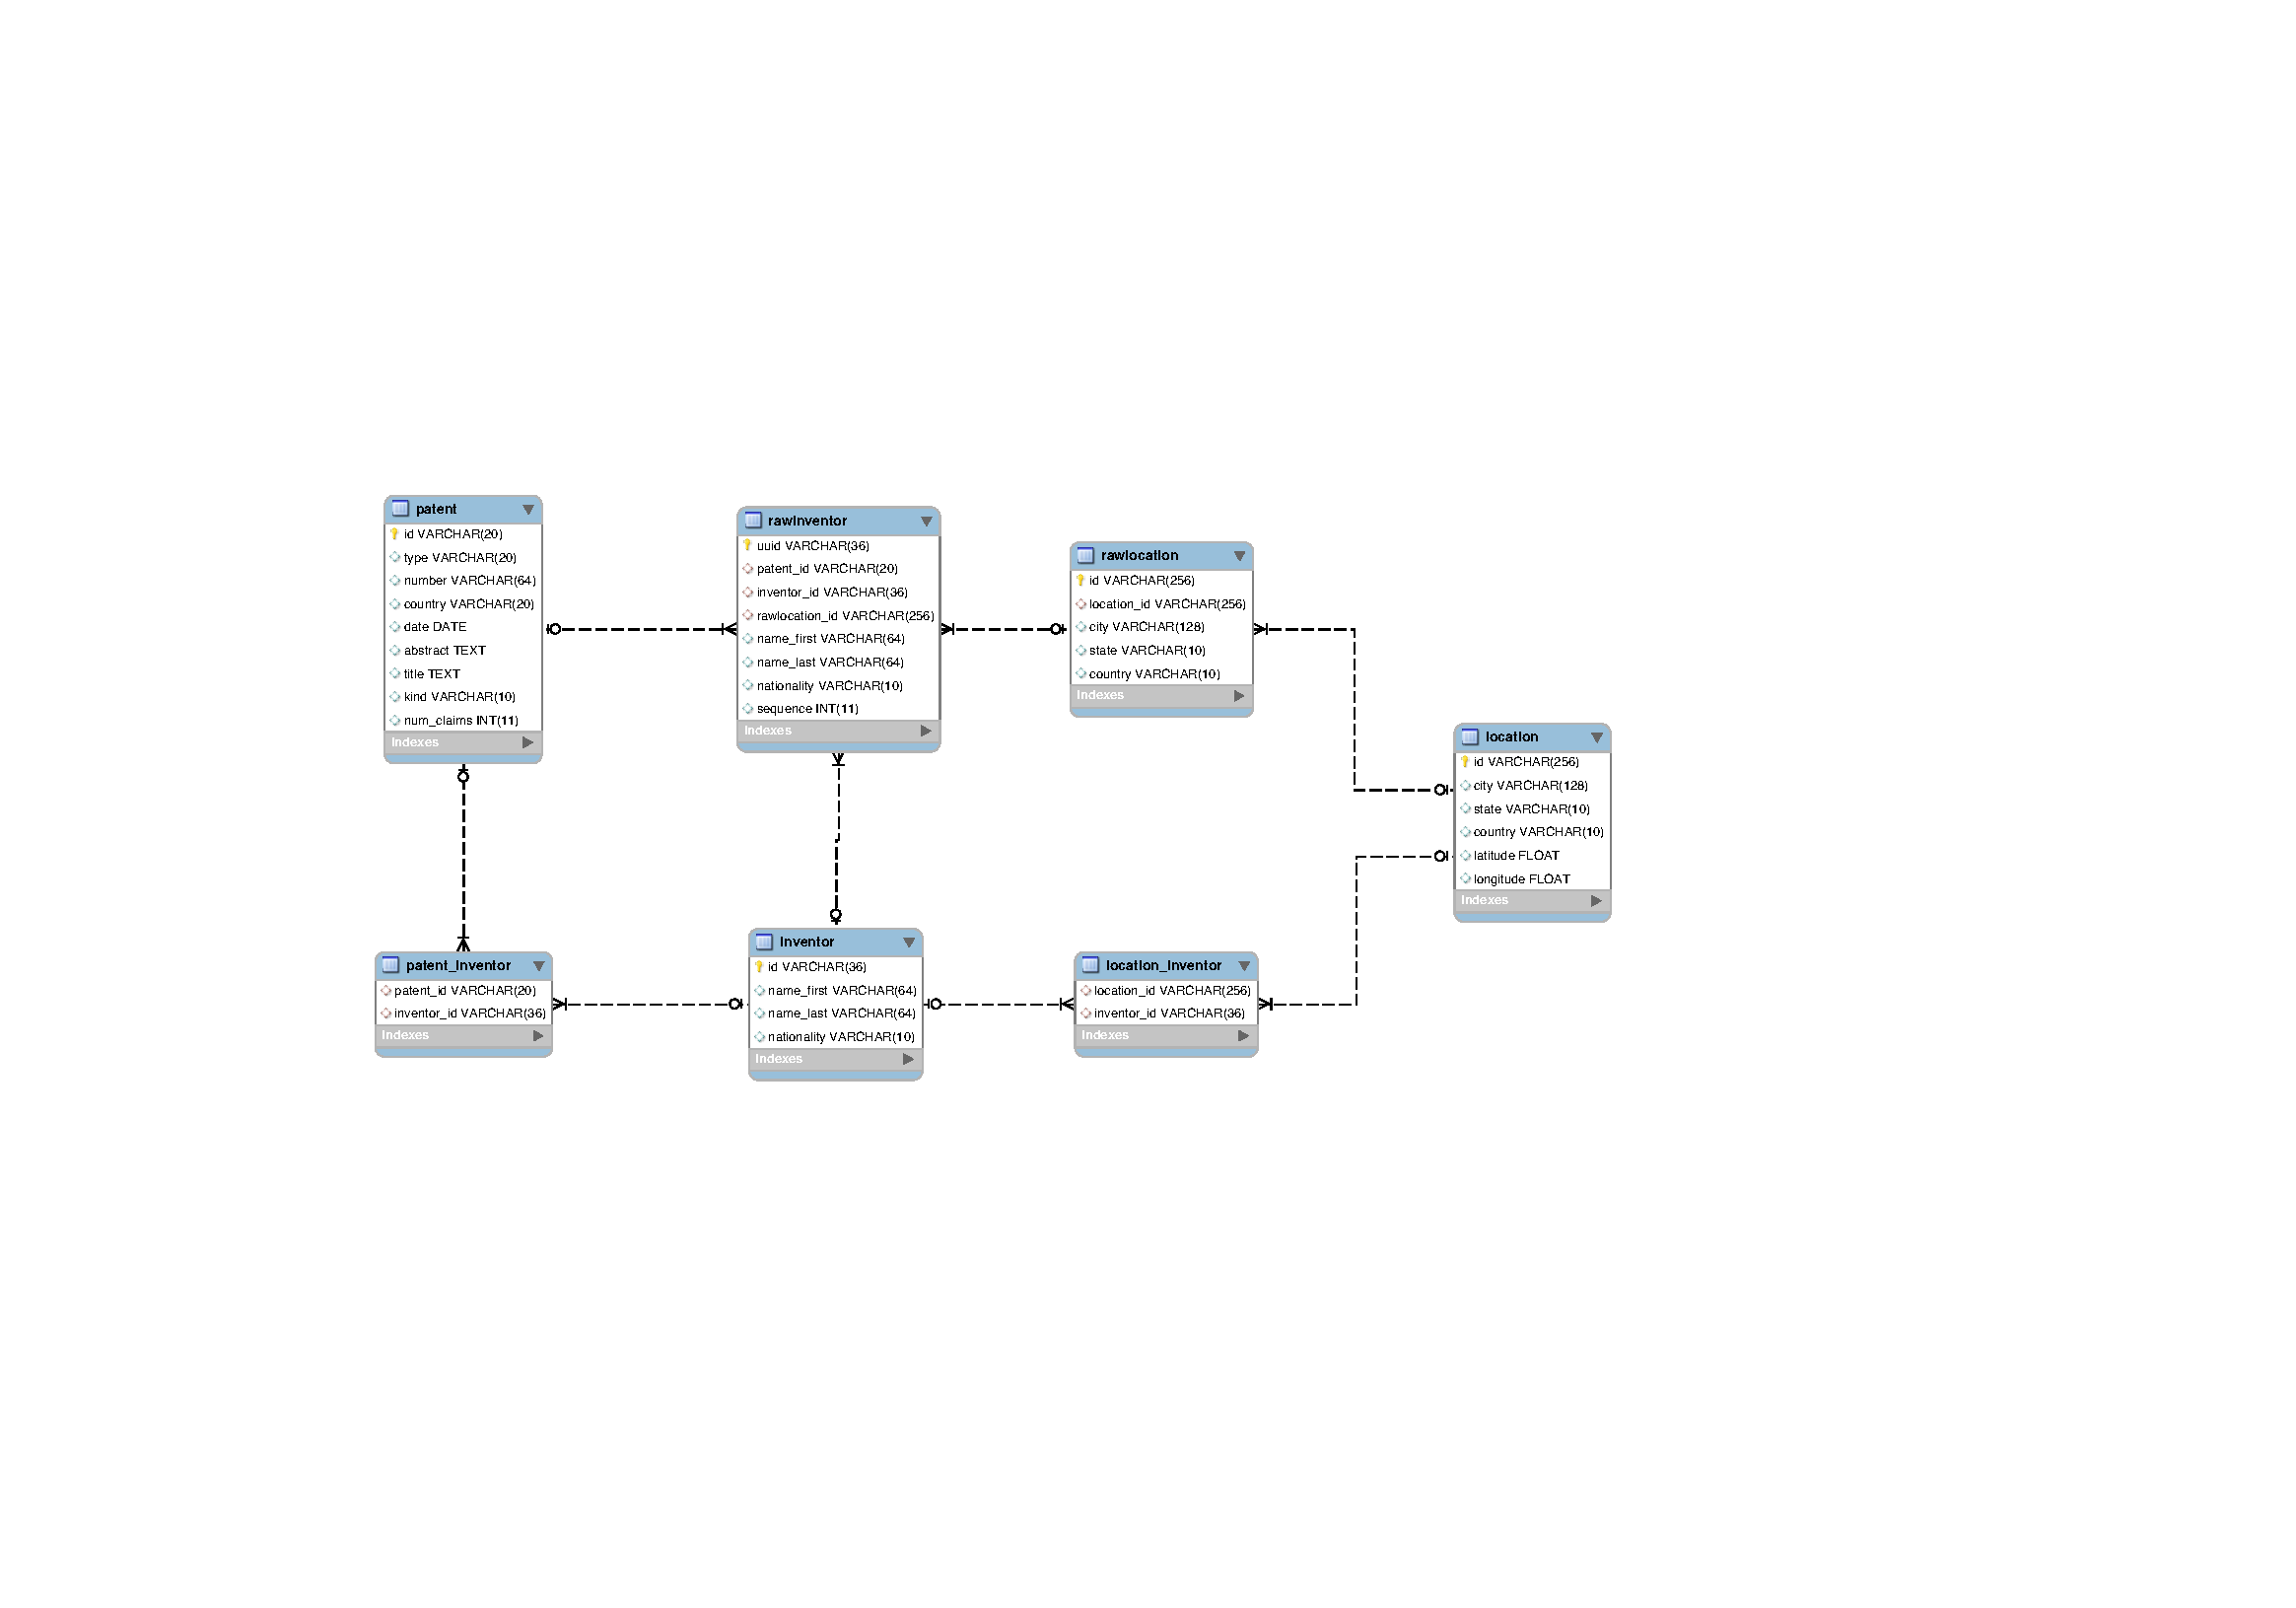
\includegraphics[width=\linewidth]{figs/Inventor}
\caption{Inventor-related tables}
\end{figure*}

\subsection*{Assignees}

The relationships between raw and disambiguated assignee records follow the same logic as the inventor records above.

\begin{figure*}[!htbp]
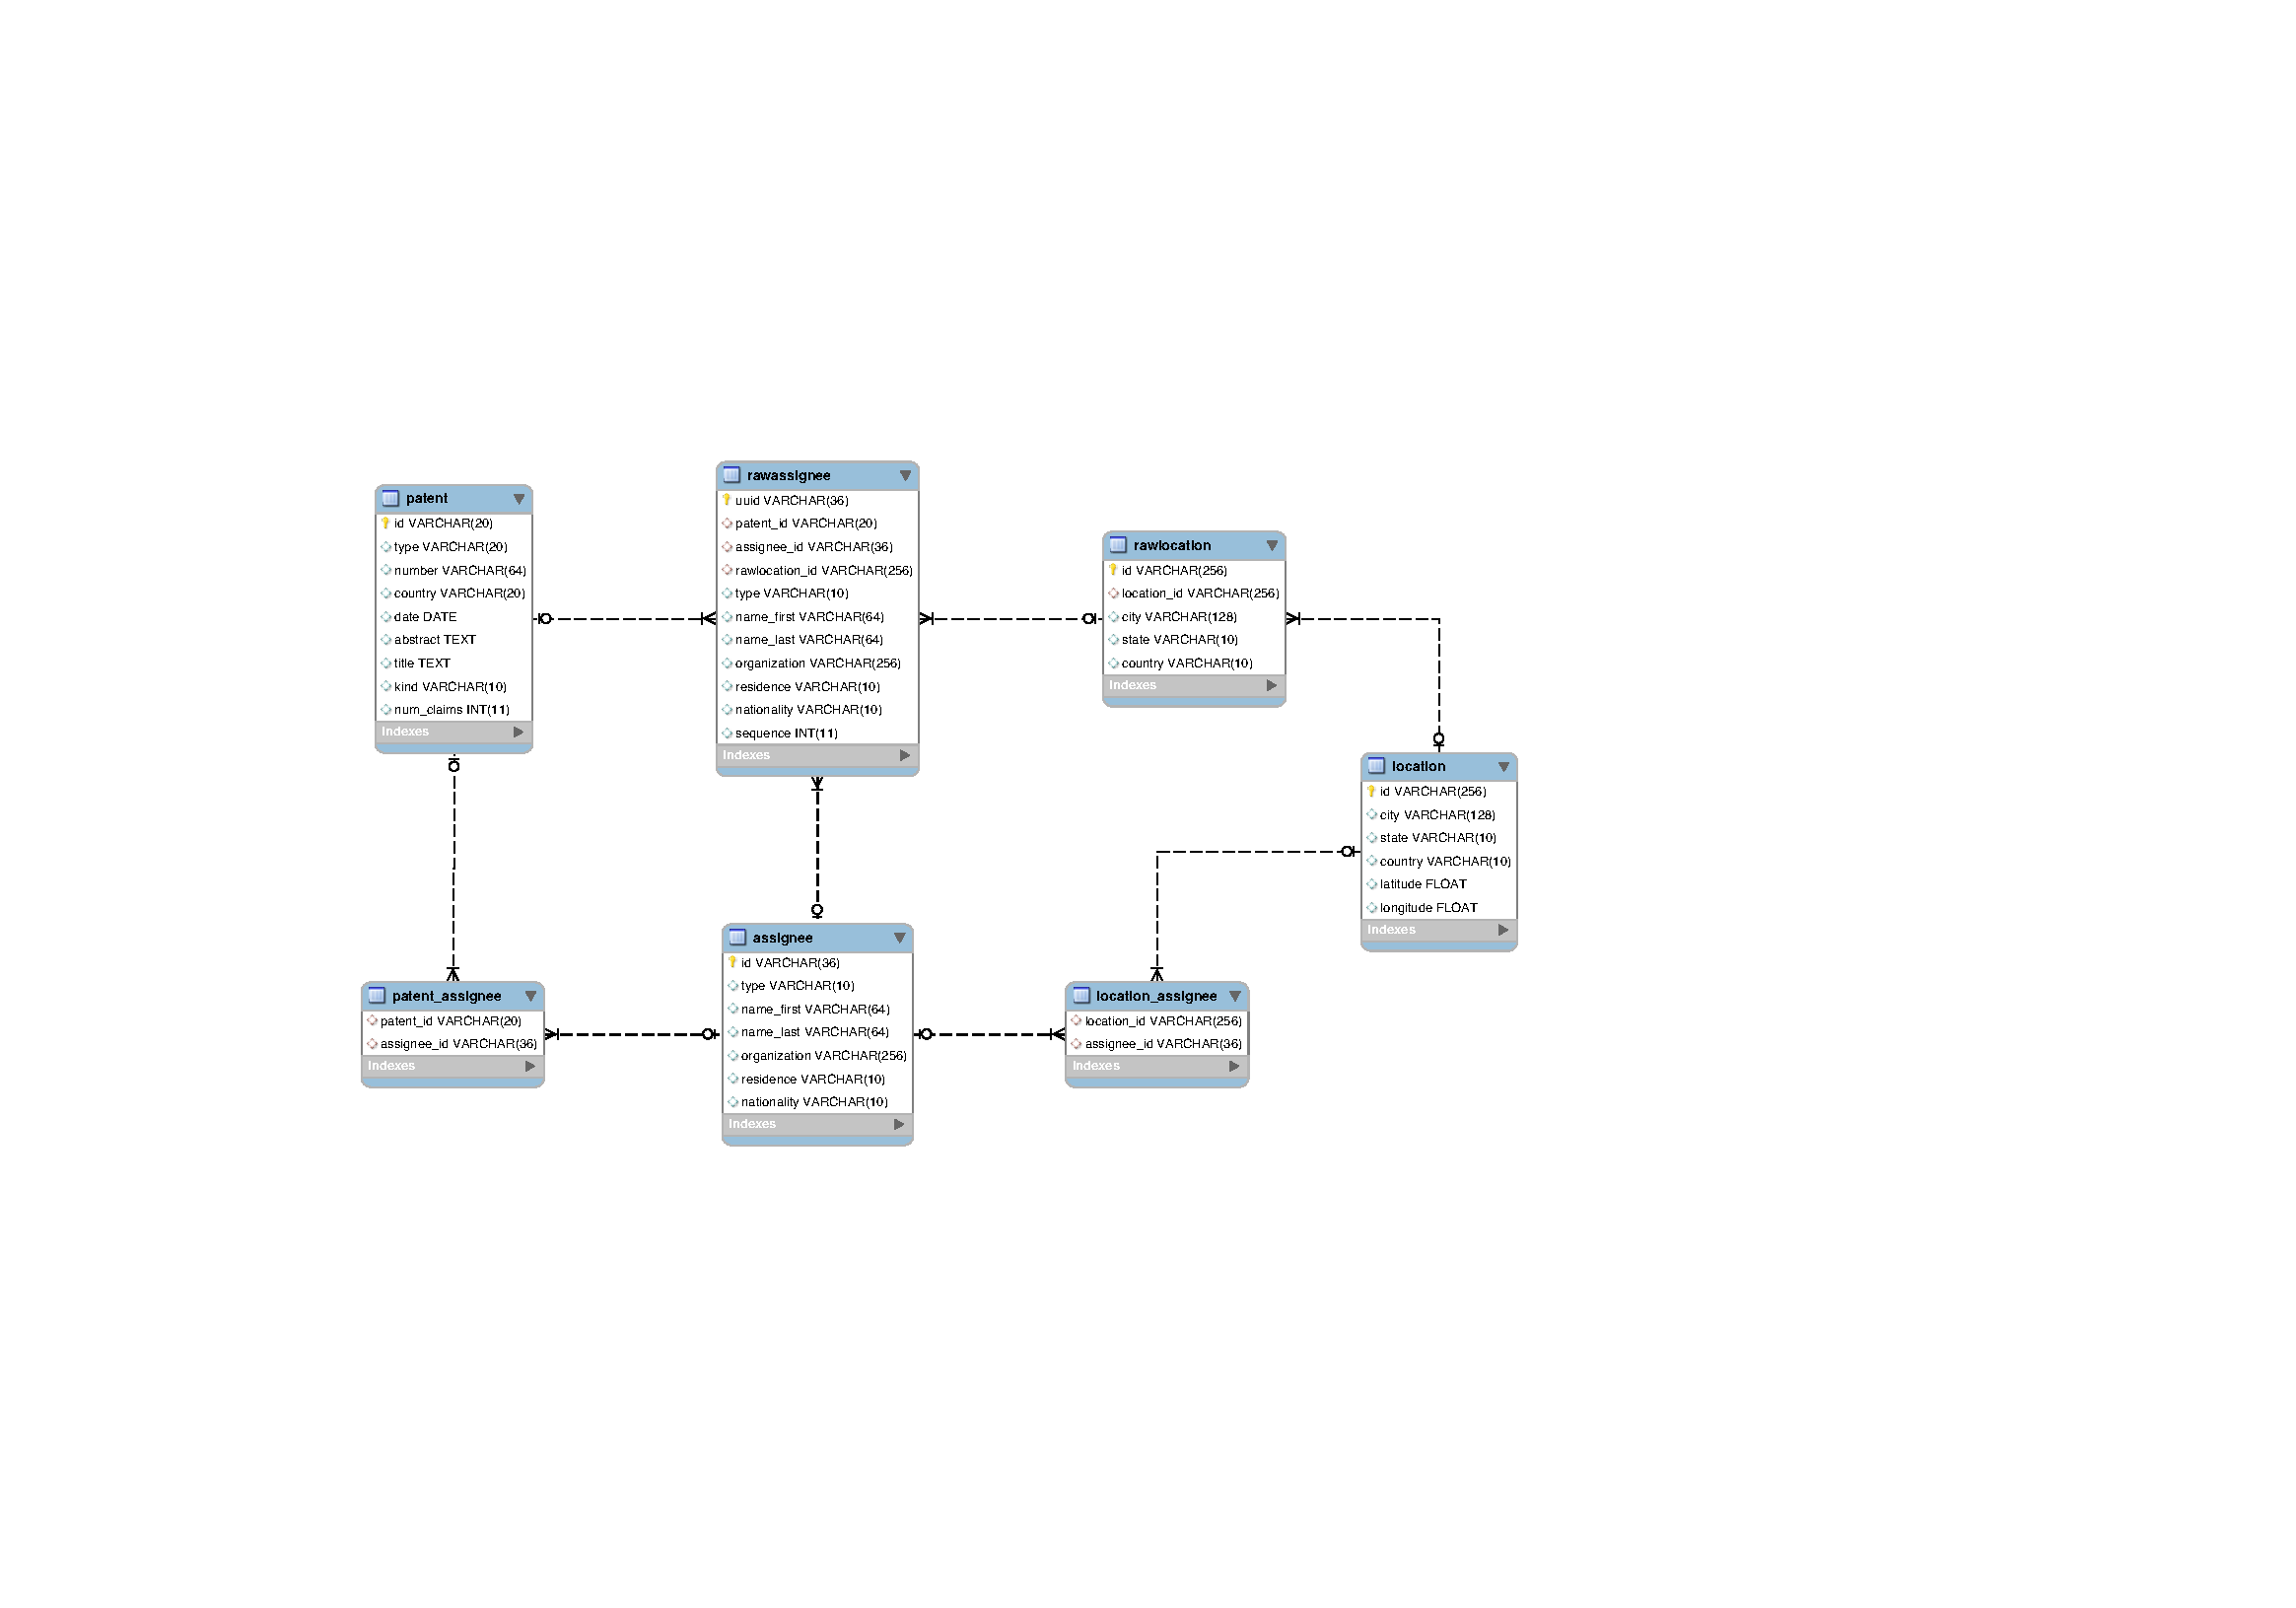
\includegraphics[width=\linewidth]{figs/Assignee}
\caption{Assignee-related tables}
\end{figure*}

\subsection*{Lawyers}

The relationships between raw and disambiguated lawyer records follow the same logic as the assignee and inventor records above, with the exception
that patent documents do not contain location information about lawyers.

\begin{figure*}[!htbp]
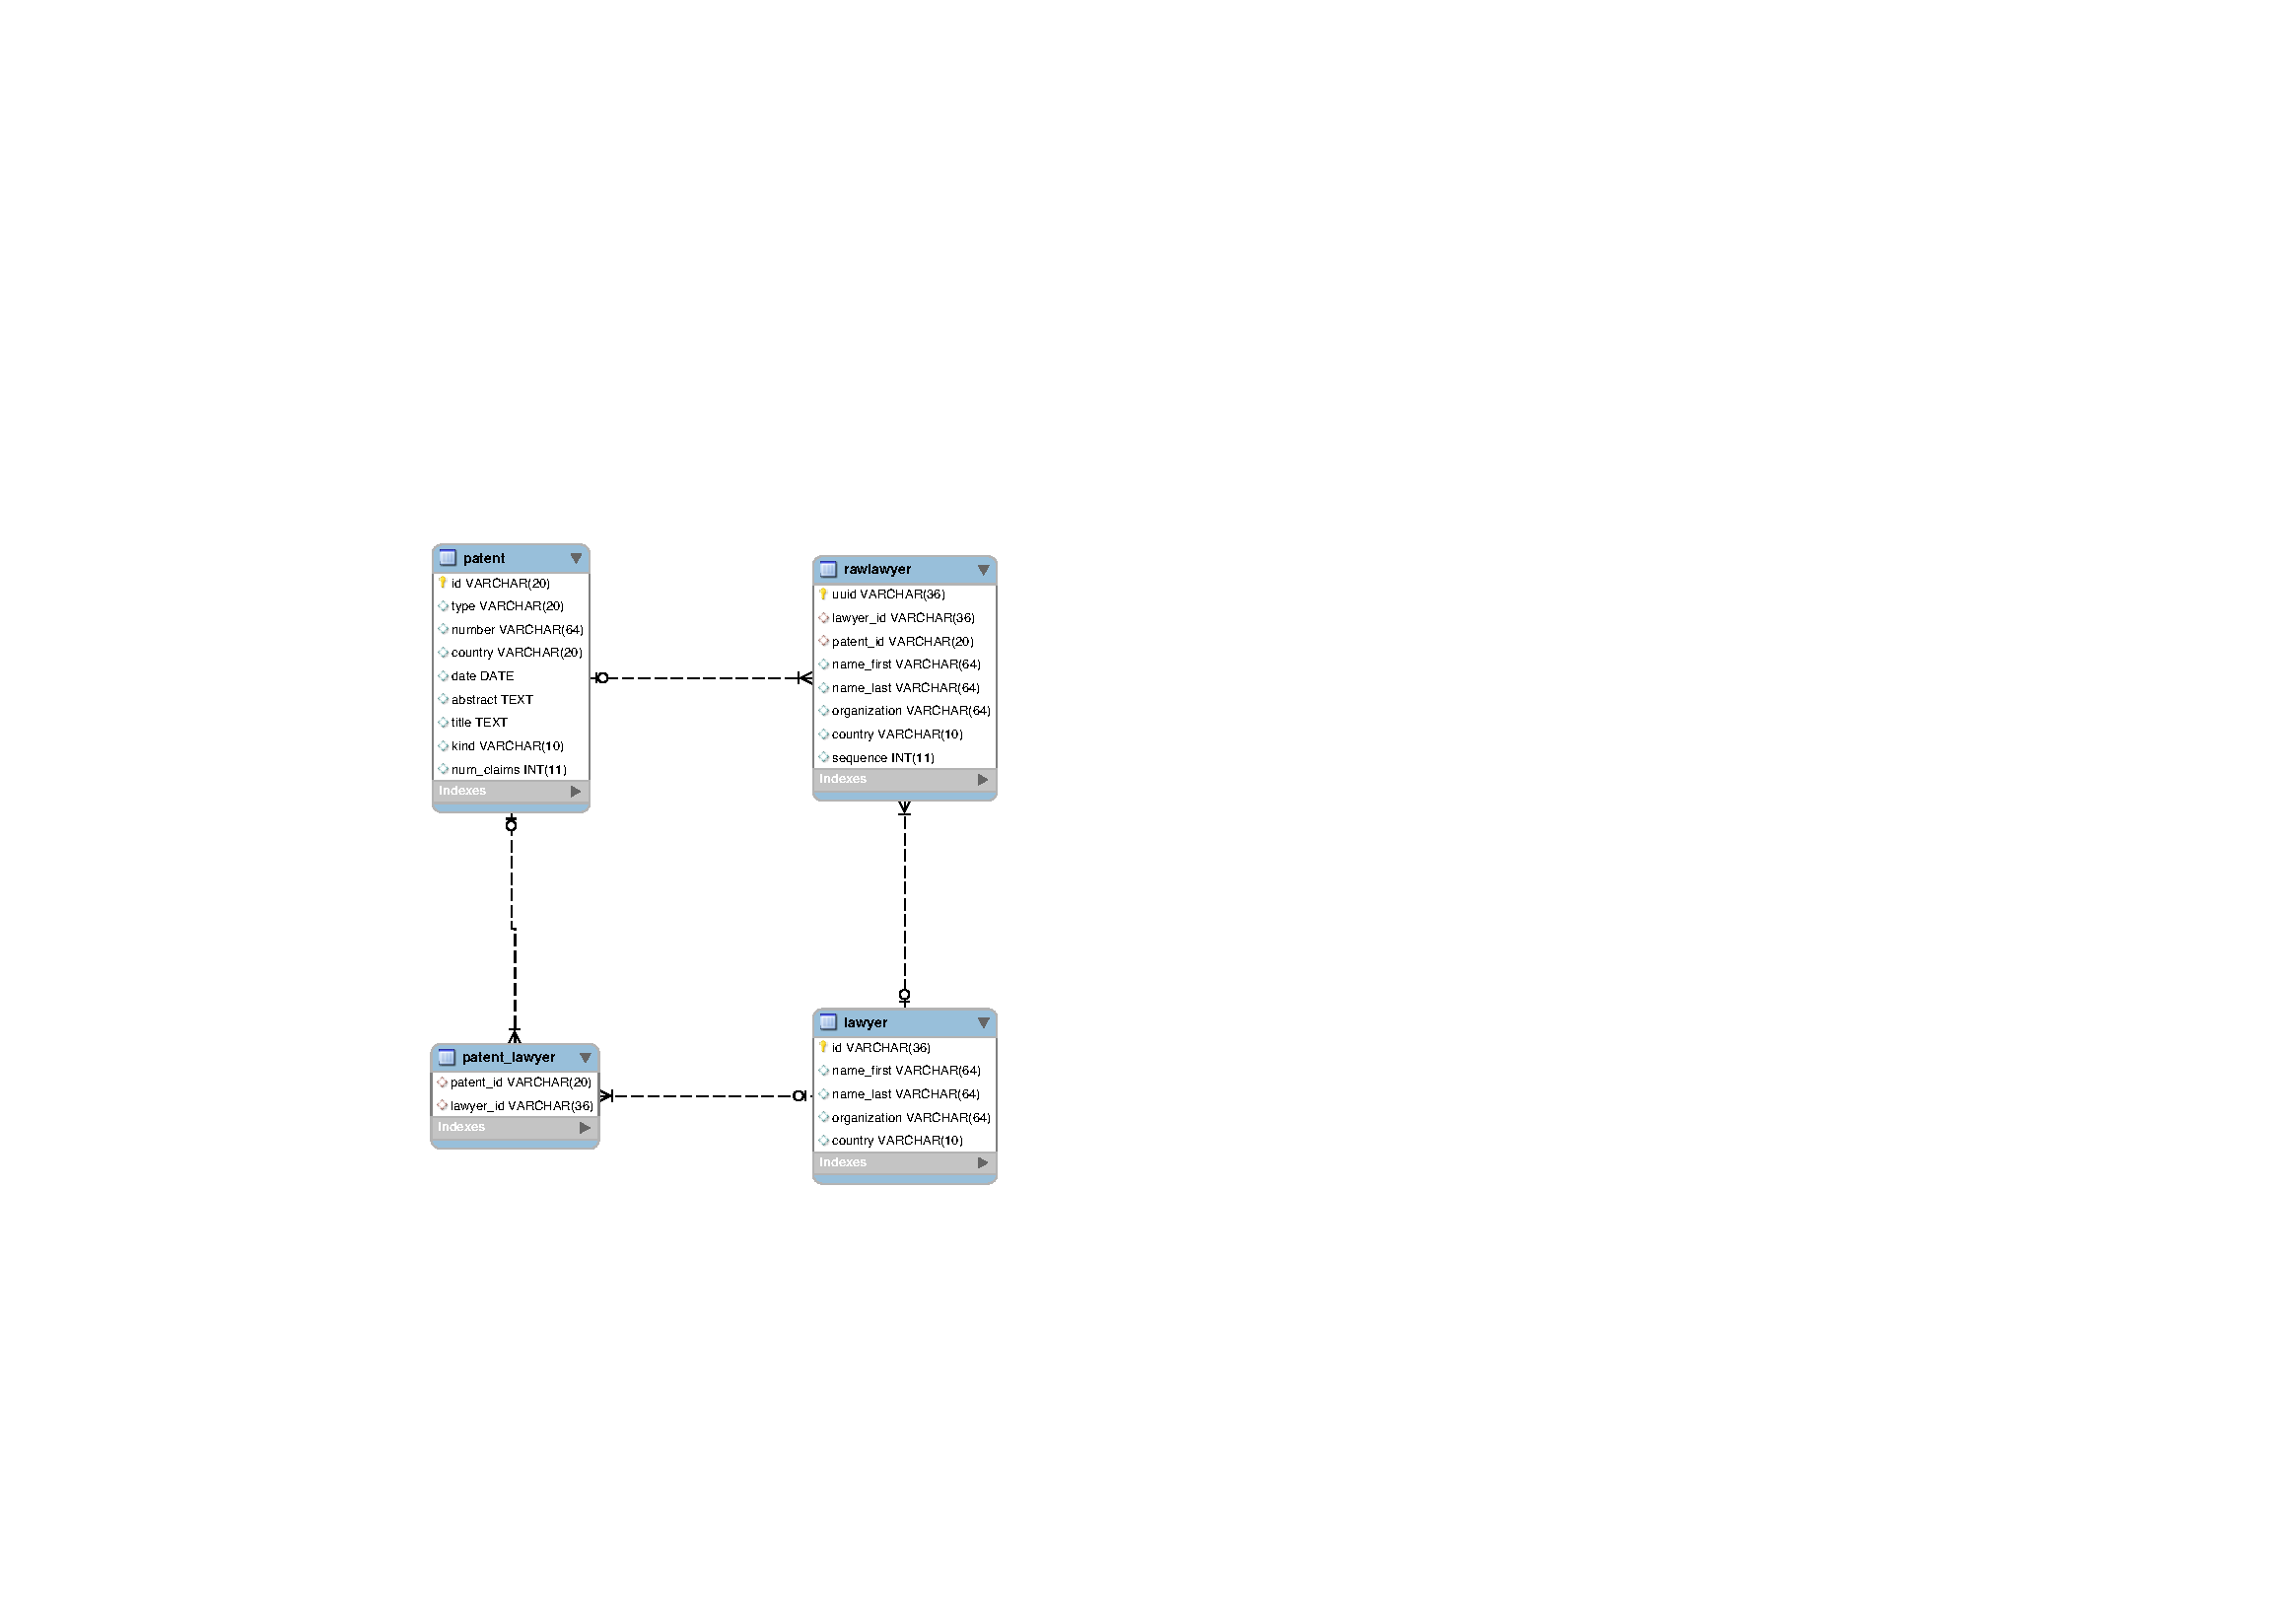
\includegraphics[width=.3\linewidth]{figs/Lawyer}
\caption{Lawyer-related tables}
\end{figure*}